\section{Analisis Kondisi Saat Ini}
\label{sec:analisis-kondisi-saat-ini}

Subbab ini membahas tentang kondisi sistem saat ini. Penulis mengidentifikasi masalah yang ada sekarang dan menggambarkan kondisi sistem saat ini pada \autoref{fig:current-state}. Dengan memahami alur kerja sistem saat ini dan mengidentifikasi keterbatasan sistem, kebutuhan fungsional dan non-fungsional sistem dapat ditentukan.

\autoref{fig:current-state} menunjukkan interaksi antara pengguna, sistem pencatatan, dan aplikasi transaksi yang digunakan saat pengguna melakukan transaksi serta pencatatan transaksi. Pengguna melakukan transaksi melalui aplikasi transaksi saat membayar tagihan. Transaksi yang dilakukan dapat berupa pembayaran menggunakan QRIS atau transfer dan menghasilkan artefak terkait. Artefak dapat berupa struk pembayaran, bukti pembayaran QRIS, atau bukti transfer. Setelah artefak dihasilkan, pengguna dan aplikasi transaksi akan menyimpan artefak transaksi tersebut. Pengguna akan mencari kembali artefak tersebut saat pengguna melakukan pencatatan transaksi. Data transaksi akan diekstrak secara manual dan disimpan dalam aplikasi pencatatan keuangan yang dimiliki.
\begin{figure}[htbp]
    \centering
    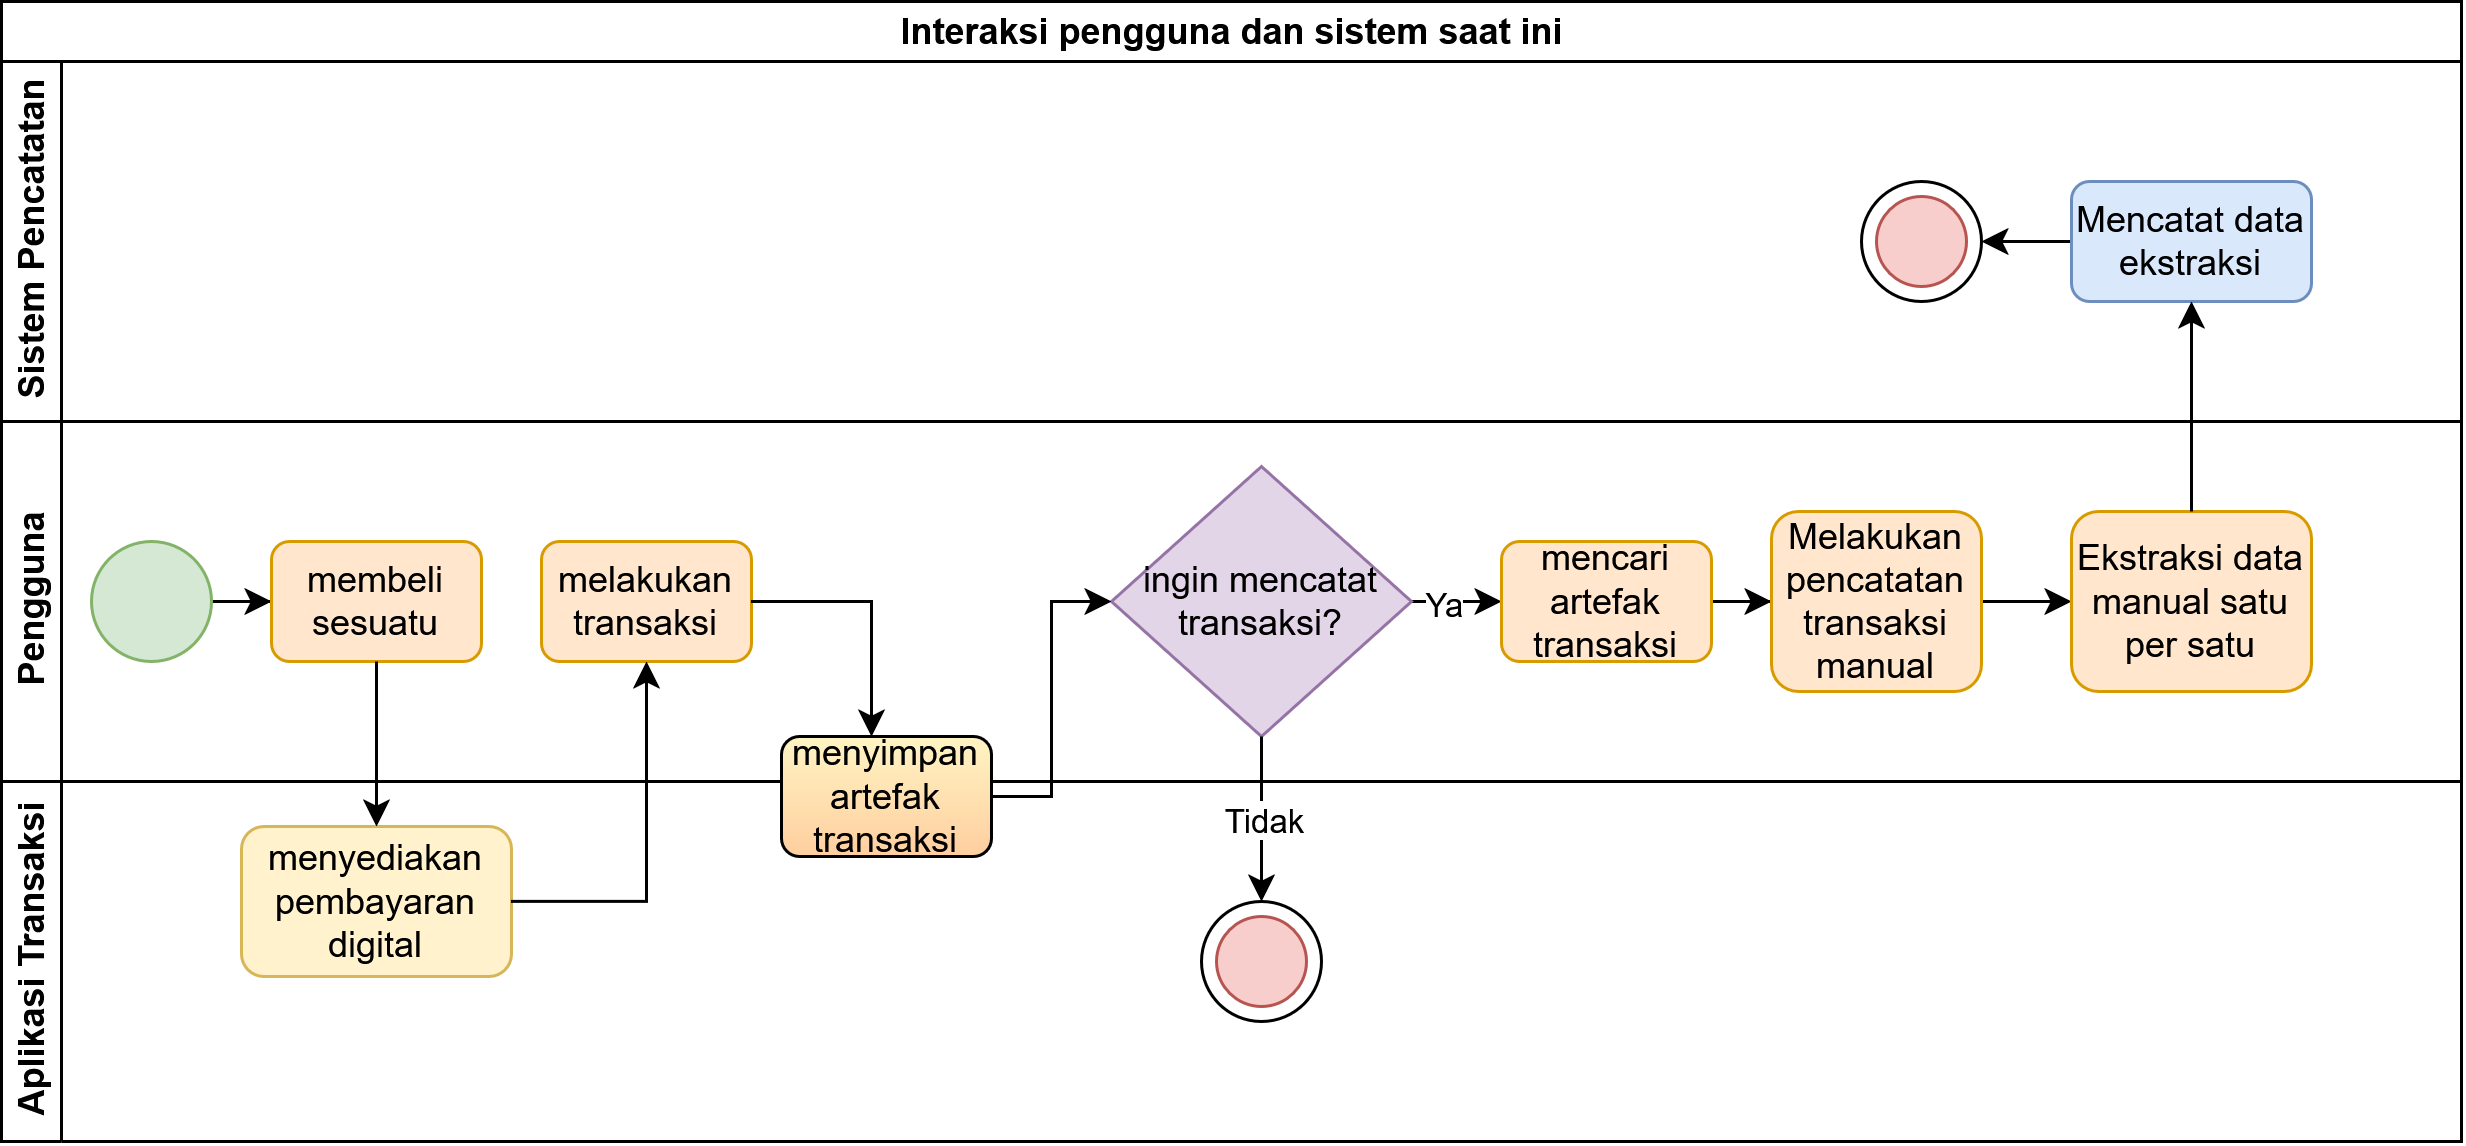
\includegraphics[width=.925\textwidth]{images/current-state.png}
    \caption{BPMN kondisi saat ini}
    \label{fig:current-state}
\end{figure}

\begin{figure}[htbp]
    \centering
    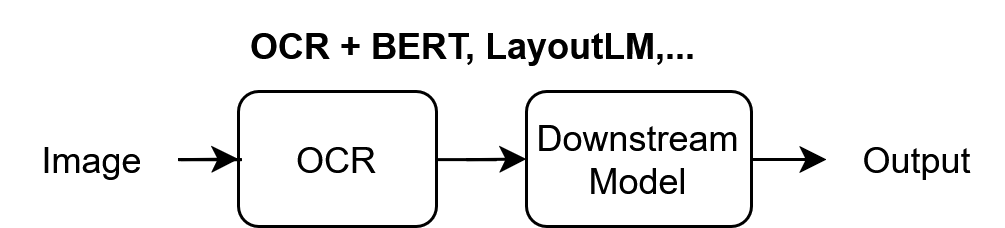
\includegraphics[width=0.8\textwidth]{images/non-donut-pipeline.png}
    \caption{\emph{Pipeline} sistem yang digunakan umumnya}
    \label{fig:non-donut-pipeline}
\end{figure}

\autoref{fig:non-donut-pipeline} menunjukkan \emph{pipeline} yang umumnya digunakan pada sistem ekstraksi data dari dokumen yang sudah menggunakan \ocr. \emph{pipeline} ini memungkinkan pengguna untuk tidak melakukan ekstraksi data secara manual. Pengguna hanya perlu mengunggah artefak yang diinginkan dan sistem akan memproses artefak tersebut dengan menggunakan \ocr. Setelah itu, sistem akan mengekstrak data dari teks yang telah didapatkan dengan menggunakan model yang telah dilatih sebelumnya. Hasil ekstraksi data akan disimpan ke dalam aplikasi pencatatan keuangan yang dimiliki pengguna.

